\documentclass[a4paper]{scrartcl}
\usepackage[utf8]{inputenc}
\usepackage[T1]{fontenc}
\usepackage{amsmath,enumerate}
\usepackage{amsfonts}
\usepackage{graphicx}
\usepackage{multicol}
\usepackage{subfig}
\usepackage{float}
\usepackage{listings}
\lstset{language=sql,basicstyle=\small,keywordstyle=\ttfamily,morekeywords={REFERENCES,DEFERRED}}
\usepackage{tabularx}
\PassOptionsToPackage{hyphens}{url}\usepackage{hyperref}
\usepackage{enumitem}

\usepackage{scrpage2}
\pagestyle{scrheadings}

\newcommand{\ul}[1]{\underline{#1}}
\newcommand{\ra}{\rightarrow}
\newcommand{\R}{\ensuremath{\mathcal{R}}}

\newtheorem{ex}{Exercise}
\newenvironment{exercise}[2]%
   {\def\tmp{}%
    \ifx\points\tmp
      \begin{ex}
    \else
      \def\tmp{1}%
      \begin{ex}[#1][#2 points\ifx\points\tmp\else \fi]
    \fi
    \normalfont
   }%
   {\end{ex} %
   }



\title{Exercise Sheet 3, 2020}
\subtitle{6.0 VU Advanced Database Systems}
\author{}

\automark{section}
\ohead{\pagemark}
\makeatletter
\chead{ADBS 2020 -- \@author}
\makeatother
\cfoot{}

\begin{document}
\maketitle





\begin{exercise}{Distributed Joins}{2}
\begin{enumerate}[label=\alph*)]
	\item 
	
	\begin{itemize}
		\item Send both tables to site 4 and join there: |Libraries| = 20,000 * 450 = 9,000,000 B, |Books| = 500,000 * 70 = 35,000,000 B. Total communication cost = |Libraries| + |Books| = 44,000,000 B.
		\item Send Libraries to site 2, join there and send the result to site 4: In general, the number of records of Libraries $\bowtie$ Books = $\frac{500000 * 20000}{50000}=200,000$. |$\pi_{info,available}$| = $200,000 * (78 + 2)=200,000 * 80=16,000,000$ B. Total communication cost = |Libraries| + |$\pi_{info,available}$| = 25,000,000 B.
		\item Symmetrically: Send Books to site 1, join there and send the result to site 4: Total communication cost = |Books| + |$\pi_{info,available}$| = 51,000,000 B.
		\item Send only the join attributes of Libraries to site 2, semi join with Books, send
		the result back to site 1 to compute the full join. Finally transfer the full join to
		site 4: |$\pi_{libid}$| = 20,000 * 16 = 320,000 B. |$\pi_{home, available}$ (Books semi join Libraries)|=200,000 * 18 = 3,600,000 B. Total communication cost = |$\pi_{libid}$| + |$\pi_{home, available}$(Books semi join Libraries)| + |$\pi_{info,available}$| = 19,920,000 B.
		\item The semi-join strategy in the opposite direction: |$\pi_{home}$| = 500,000 * 16 = 8,000,000 B. |$\pi_{libid, info}$(Libraries semi join Books)|=10,000 * (16+78) = 940,000 B. Total communication cost = |$\pi_{home}$| + |$\pi_{libid, info}$ (Books semi join Libraries)| + |$\pi_{info,available}$| = 25,740,000 B.
	\end{itemize}
	
	Adapting to early projecting leads to decreased costs for the initial three strategies, with the second strategy even outperforming the fifth strategy:
	
	\begin{itemize}
		\item Send both tables to site 4 and join there: |$\pi_{libid, info}$| $= 20,000 * (16+78) = 1,880,000$ B, |$\pi_{home, available}$| $= 500,000 * (16+2) = 9,000,000$ B. Total communication cost = |$\pi_{libid, info}$| + |$\pi_{home, available}$| = 10,880,000 B.
		\item Send Libraries to site 2, join there and send the result to site 4: Total communication cost = |$\pi_{libid, info}$| + |$\pi_{info,available}$| = 17,880,000 B.
		\item Symmetrically: Send Books to site 1, join there and send the result to site 4: Total communication cost = |$\pi_{home, available}$| + |$\pi_{info,available}$| = 25,000,000 B.
	\end{itemize}

	In general, one sees that simply transferring both projected table to site 4 is the optimal way. For the other strategies it is apparant that bringing Libraries to Books is preferable, as less records have to be transmitted. Also, the semi join is better than directly joining on table the the site of the other if the transmitted table is small enough.

\item 
For the join between Libraries and Books, directly sending it to site 4 is optimal, as described above. Thus, the communication cost for $\pi_{info,bid}$ (Libraries $\bowtie_{{libid,home}}$ Books) is 1,880,000 + 12,000,000 = 13,880,000 B.

Another contender would be to use a semi join by transferring Libraries. Since |$\pi_{info, bid}$("inner join")| = 200,000 * (78+8)=17,200,000, this would result in 320,000 + 4,800,000 + 17,200,000=22,320,000 B. All other strategies are suboptimal, as explained above.

For the outer join, since all attributes of Reviews are needed in the output and since the selectivity is $\frac{1}{1200}$, the strategy of simply sending Reviews to site 4 is optimal. |Reviews| = 1,200 * 5,000 = 6,000,000 B. Therefore, for the whole query: |Reviews $\bowtie$ $\pi_{info, bid}$("inner join")|= |Reviews| + |$\pi_{info, bid}$("inner join")| = 19,880,000 B.

\end{enumerate}
\end{exercise}


\begin{exercise}{Denormalization}{3}
The guiding principle is not to embed the Borrowed relation into another one, since it is updated frequently.
	
Denormalization might be benefitial since server-side joins are not supported. Since the Person collection is not updated often and is only used by the Borrowed collection, it can be denormalized. This way, the first query can be quickly executed without any join. Since a Borrowed document contains exactly one Person, it can even be directly embedded. It could also be argued that the first query does not necessarily ask for a persons address, hence only the name would need to be denormalized, which would result in the name simply being a reference to the Person document.

Book and Edition form an 1:n relationship. Both relations are updated seldomly. Thus, Edition can be denormalized by embedding each Edition record into an \texttt{editions} list of a Book record. This increases the second query performance, since an application-side join is not needed anymore to get the sum of \texttt{owned} for each book. What is still needed for this query is that both Book and Borrowed need to be checked. This can not be circumvented by embedding Book into Borrowed, since Borrowed can contain multiple records for each book.


For the JSON files, the fourth row of the Borrowed table is chosen as example instance and can be seen in \texttt{borrowed.json} and \texttt{book.json}.
\end{exercise}

\begin{exercise}{Graph Databases}{5}

\begin{enumerate}[label=\alph*)]
\item 

Either \texttt{countries} or \texttt{country\_codes} could be used. The three queries are:


\begin{verbatim}
match (a:Address) return distinct a.countries;

match (a:Address) return distinct a.countries, count(a.countries);

match (o:Officer) -[:REGISTERED_ADDRESS]-> (:Address {countries:'Japan'})
return distinct o limit 5;
\end{verbatim}

\item \label{it:5b}

Surely it will not make a difference whether \texttt{count(*)} appears once with as or multiple times, as the query optimizer will optimize this in the latter case. Anyway, both variants are used in the below queries. 
\begin{verbatim}
match (i:Intermediary) -[e:INTERMEDIARY_OF]-> ()
with i, count(e) as edgeCount order by edgeCount desc
return i, edgeCount limit 20;

match (i:Intermediary) -[m:INTERMEDIARY_OF]-> (), (i) -[o:OFFICER_OF]-> ()
return i.name, count(m), count(o)
order by count(m) + count(o) desc limit 20;

match (i:Intermediary) -[m:INTERMEDIARY_OF]-> (), (i) -[o:OFFICER_OF]-> ()
with i, count(m) as mCount, count(o) as oCount
order by mCount + oCount desc limit 1
match (i) -[e]-> (x)
where type(e) <> "INTERMEDIARY_OF" and type(e) <> "OFFICER_OF" return i, e, x;
\end{verbatim}

The result can be seen in \autoref{fig:5b}.

\begin{figure}[h]
\centering

\includegraphics[height=.18\textheight]{b3}
\caption{Result of query \ref{it:5b}}
\label{fig:5b}
\end{figure}

\item \label{it:5c}

In this case, one could either determine the max length using \texttt{length(p) <= 30} or using the \texttt{minHops..maxHops} functionality of paths. Assuming that the latter might be more optimized it is used in the below query.

\begin{verbatim}
match p=shortestPath((l:Address {countries: 'Luxembourg'}) -[*0..30]-
(c:Address {countries: 'Cyprus'}))
where length(p) >= 16 return p limit 1;
\end{verbatim}

The result can be seen in \autoref{fig:5c}.

\begin{figure}[h]
	\centering
	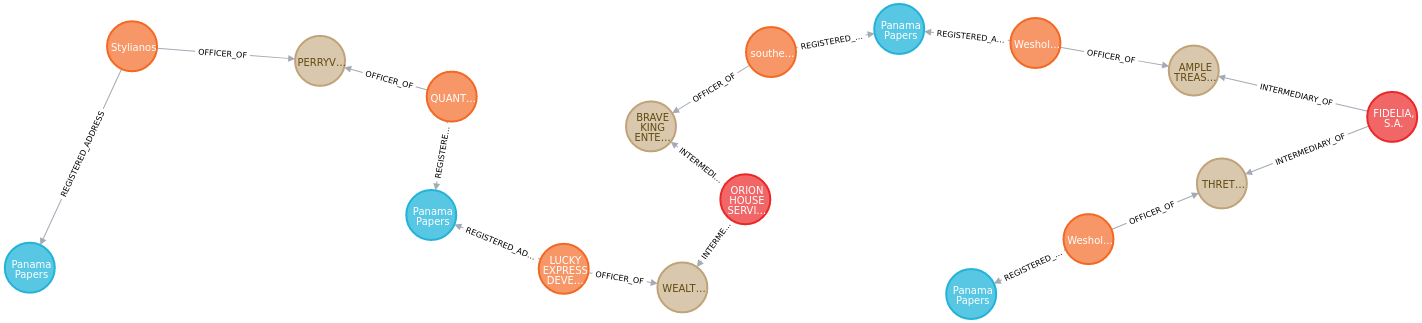
\includegraphics[width=\textwidth]{c}
	\caption{Result of query \ref{it:5c}}
	\label{fig:5c}
\end{figure}

\item \label{it:5d}

The query is quite straightforward and makes use of the possibility of matching multiple relationships.

\begin{verbatim}
match
(i:Intermediary) -[:INTERMEDIARY_OF]-> (e:Entity) <-[:OFFICER_OF]- (o:Officer),
(i) -[:INTERMEDIARY_OF]-> (e2:Entity) <-[:OFFICER_OF]- (o)
where e.countries <> e2.countries and
(e.jurisdiction <> e.country_codes or e2.jurisdiction <> e2.country_codes)
return * limit 1;
\end{verbatim}

The result can be seen in \autoref{fig:5d}.

\begin{figure}[h]
	\centering
	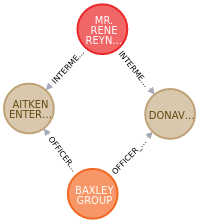
\includegraphics[height=.25\textheight]{d}
	\caption{Result of query \ref{it:5d}}
	\label{fig:5d}
\end{figure}

\item \label{it:5e}

First, as a safety measure, add a constraint on \texttt{COUNTRIES} to ensure that no duplicate countries are created.

\begin{verbatim}
create constraint on (c:COUNTRY) assert (c.name) is unique;
\end{verbatim}

Now, since a country is unique and merge only creates a relationship if no prior relationship is found, following query works:

\begin{verbatim}
match (o:Other) where o.countries is not null and not o.countries contains ';' merge (c:COUNTRY {name: o.countries}) merge (o)-[:IN_COUNTRY]->(c) return c;
\end{verbatim}

Finally, all nodes connected to Japan can be found using the below query and seen in \autoref{fig:5e}.

\begin{verbatim}
match (c:COUNTRY {name: 'Japan'}) <-[:IN_COUNTRY]- (o) return *;
\end{verbatim}

\begin{figure}[h]
	\centering
	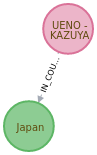
\includegraphics[height=.2\textheight]{e}
	\caption{Result of query \ref{it:5e}}
	\label{fig:5e}
\end{figure}


\end{enumerate}

  
\end{exercise}


\end{document}
